\documentclass[final]{elsarticle}

\usepackage{setspace}\doublespacing

\usepackage{graphicx}
\usepackage{tikz}
\usepackage{amsmath} 
\usepackage{amssymb}
\usepackage{amsthm}
\usepackage{units}   
\usepackage{float}   
\usepackage{graphicx}
\usepackage{amsfonts}
\usepackage{mathrsfs}
\usepackage[colorlinks]{hyperref}
\usepackage{framed}
\usepackage{url}

\floatstyle{ruled}
\newfloat{program}{thp}{lop}
%-------------------------------------------
\newcommand{\sign}{\ensuremath{\mathrm{sign}}}
\newcommand{\diag}{\ensuremath{\mathrm{diag}}}
\newcommand{\trace}[1]{\ensuremath{\mathrm{trace}\left( #1 \right)}}
\newcommand{\norm}[1]{\ensuremath{\left\|#1\right\|_2^2}}
\newcommand{\func}[2]{\ensuremath{\mathrm{#1}\left( #2 \right)}}
\newcommand\eps \epsilon
\newcommand{\R}{\ensuremath{\mathbb{R}}}
\newcommand{\N}{\ensuremath{\mathbb{N}}}
\newcommand{\real}{\ensuremath{\mathbb{R}}}
\newcommand{\cl}[1]{\ensuremath{\mathcal{#1}}}
\newcommand{\suppsize}[1]{\ensuremath{|\mathcal{#1}|}}
\newcommand{\vect}[1]{\ensuremath{\mathbf{#1}}}
\newcommand{\matr}[1]{\ensuremath{\mathbf{#1}}}
\newcommand{\deriv}[2]{\frac{\partial #1}{\partial #2}}
\newcommand{\arr}[2]{\begin{array}{#1}#2\end{array}}
\newcommand{\mat}[2]{\left(\begin{array}{#1}#2\end{array}\right)}
\newcommand{\brc}[2]{\left\{\begin{array}{#1}#2\end{array}\right.}
\newcommand{\pars}[1]{\left(#1\right)}
\newcommand{\brcs}[1]{\left\{#1\right\}}
\newcommand{\half}{\frac{1}{2}}

% Bold symbols and operators
\newcommand\Laplacian{\nabla^2}
\newcommand\bnabla{\boldsymbol{\nabla}}
\newcommand\bLaplacian{\boldsymbol{\nabla}^2}
\newcommand\bcdot{\boldsymbol{\cdot}}
\newcommand\bU{\mathscr{\boldsymbol{U}}}
\newcommand\bv{\boldsymbol{v}}
\newcommand\bV{\boldsymbol{V}}
\newcommand\bE{\boldsymbol{E}}
\newcommand\be{\boldsymbol{\hat{e}}}
\newcommand\bn{\boldsymbol{\hat{n}}}
\newcommand\bk{\boldsymbol{\hat{k}}}
\newcommand\bj{\boldsymbol{j}}
\newcommand\bi{\boldsymbol{i}}
\newcommand\bs{\boldsymbol{s}}
\newcommand\bA{\boldsymbol{A}}
\newcommand\bF{\boldsymbol{F}}
\newcommand\bG{\boldsymbol{G}}
\newcommand\bI{\boldsymbol{I}}
\newcommand\bJ{\boldsymbol{J}}
\newcommand\bx{\boldsymbol{x}}
\newcommand\by{\boldsymbol{y}}
\newcommand\bz{\boldsymbol{z}}
\newcommand\br{\boldsymbol{r}}
\newcommand\bc{\boldsymbol{c}}
\newcommand\bxhat{\hat{\bx}}
\newcommand\byhat{\hat{\by}}
\newcommand\bzhat{\hat{\bz}}
\newcommand\brhat{\hat{\br}}
\newcommand\bnhat{\hat{\boldsymbol{n}}}
\newcommand\btheta{\boldsymbol{\theta}}
\newcommand\bthetahat{\hat{\btheta}}
\newcommand\bphi{\boldsymbol{\phi}}
\newcommand\bphihat{\hat{\bphi}}
\newcommand\bzero{\boldsymbol{0}}
\newcommand\bomega{\boldsymbol{\omega}}
\newcommand\bpsi{\boldsymbol{\psi}}

% Calligraphic symbols
\newcommand\cB{\mathcal{B}}
\newcommand\cE{\mathcal{E}}
\newcommand\cF{\mathcal{F}}
\newcommand\cO{\mathcal{O}}
\newcommand\cG{\mathcal{G}}
\newcommand\cI{\mathcal{I}}
\newcommand\cP{\mathcal{P}}
\newcommand\cD{\mathcal{D}}
\newcommand\cL{\mathcal{L}}
\newcommand\cU{\mathscr{U}}
\newcommand\cV{\mathscr{V}}
\newcommand\cW{\mathscr{W}}

% Tensors
\newcommand\tI{\mathsf{I}}
\newcommand\tS{\mathsf{S}}
\newcommand\tT{\mathsf{T}}

% Unit vector
\newcommand\ui{\boldsymbol{\hat{\imath}}}

\setlength{\textheight}{8.7in}
\setlength{\columnsep}{2.0pc}
\setlength{\textwidth}{6.6in}
% \setlength{\footheight}{0.2in}
\setlength{\topmargin}{0.05in}
\setlength{\headheight}{0.2in}
\setlength{\headsep}{0.1in}
\setlength{\evensidemargin}{0in}
\setlength{\oddsidemargin}{0in}
% \setlength{\parindent}{1pc}
\setlength{\parindent}{0.0 in}
\setlength{\parskip}{0.1 in}


\journal{Journal of Computational Physics}

\begin{document}

\begin{frontmatter}

\title{Numerical and asymptotic solution of nonlinear electrokinetic phenomena}
\author[cs]{Roman Zeyde}
\author[cs]{Irad Yavneh}
\author[math]{Ehud Yariv}

\address[cs]{Department of Computer Science, Technion -- Israel Institute of Technology, 
Haifa 32000, Israel}
\address[math]{Department of Mathematics, Technion -- Israel Institute of Technology, 
Haifa 32000, Israel}

\begin{abstract}
\end{abstract}

\begin{keyword}
numerical, solver, electrokinetics, nonlinear
\end{keyword}

\end{frontmatter}


%%%%%%%%%%%%%%%%%%%%%%%%%%%%%%%%%%%%%%%%%%%%%%%%%%%%%%%%%%%%%%%%%%%%%%%%%%%%%%%%%%%%%%%%%%%%%%%%%
\section{Introduction} \label{sec:intro}

Electrokinetic theory describes the dynamics of charged particles
in ionic fluids \cite{kirby2010book}.
When a particle acquires surface charge, a layer
of ions of opposite charge is attracted to the surface via    
electric forces, creating a double-layer structure around the
particle (see Figure \ref{fig:EDL}). This structure, called
``Debye layer'', electrically screens the surface charge, thus
creating a potential difference between the particle and the outer
layer of the fluid bulk.
In cases where the layer width is much smaller than the particle's
size, an analytical asymptotic solution for the Debye layer
dynamics can be found \cite{yariv2010asymptotic}.

\begin{figure}[htbp]
    \begin{center}
        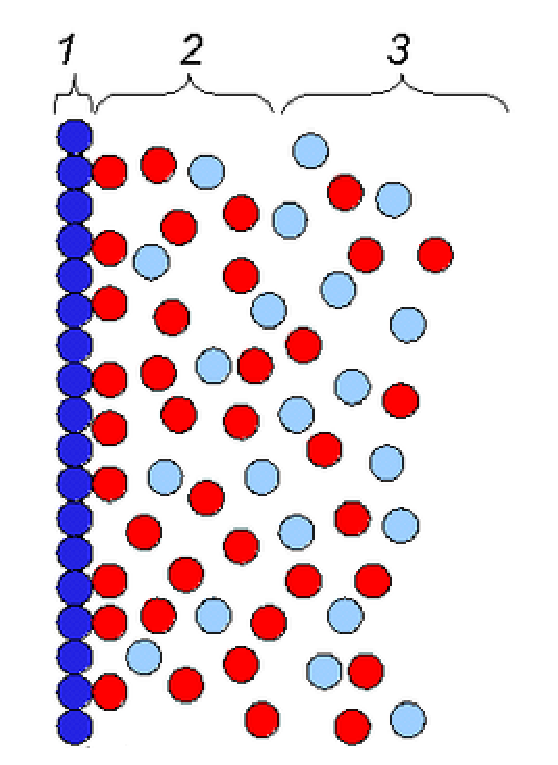
\includegraphics[width=0.2\textwidth]
            {figs/ElectricDoubleLayer.eps}
        \caption{Schematic structure of the double layer:
        (1) particle surface, (2) Debye layer, (3) fluid bulk.
        If the particle surface has positive (blue) surface charge,
        it attracts negative (red) ions from the fluid making the
        Debye layer negatively charged (as opposed to the rest of
        the fluid bulk, which is electrically neutral).
        The zeta potential is defined as the voltage drop across (2).}
        \label{fig:EDL}
    \end{center}
\end{figure}
% \begin{tikzpicture}\end{tikzpicture}

The variables of the electrokinetic problem are the electrostatic
potential $\varphi$, fluid velocity $\bv$ and its pressure $p$, and
ionic concentration $c$.
The boundary conditions are determined by the specific
problem under consideration and defined by the particle's
geometry, chemical characteristics, and the fluid dynamics.
The partial differential equations that describe the system dynamics
under an external electric field, are coupled and nonlinear, and
in general they have no analytic solution. 
Moreover, any numerical solver must handle the scale disparity caused by the
Debye layer width being much smaller than the particle's size. 

A closed-form linear asymptotic solution has been developed for
spherical ion-exchanging particles and weak electric field in an
axisymmetric setting \cite{yariv2010migration} but it is hard to extend this
analytic solution to more general systems. Once the electric field
becomes stronger, significant nonlinear phenomena are expected.
This interesting regime has not yet been explored.
Recently, it has been conceived that such type of dynamics
can be very useful in transporting and manipulating micro-
and nanoscale objects in many nanotechnology applications,
such as the self-assembly of superstructures, roving sensors, 
drug-delivery systems and useful nanomachinery 
\cite{howse2007self,paxton2004catalytic,pumera2010electrochemically}.
However, since the model for these electrokinetic
phenomena has no closed-form analytic solution, a numerical
solver for this system is of importance.

The goal of this work is to develop and implement an iterative numerical
solver for nonlinear electrokinetic problems, and apply it to the study
of systems that have no closed-form solutions.
This solver can be used to gain insight into the chemical and physical behavior 
in far more general regimes than are currently well-understood, 
and also to possibly lead to further analytical developments, based on new scaling behavior
discovered numerically. We may also target interesting physical
phenomena that have been observed experimentally.

The paper is structured as follows: the governing equations of the electrokinetic model
are derived in Section \ref{sec:equations}. The algorithm for the discretization and 
the solution of the system is described in Section \ref{sec:algorithm}.
The analytical asymptotic solution for the non-linear system is derived 
and presented in Section \ref{sec:asymp}.
The numerical results and their comparison to the analytical asymptotic solution 
are presented and discussed in Section \ref{sec:results}. 

%%%%%%%%%%%%%%%%%%%%%%%%%%%%%%%%%%%%%%%%%%%%%%%%%%%%%%%%%%%%%%%%%%%%%%%%%%%%%%%%%%%%%%%%%%%%%%%%%
\section{Governing Equations} \label{sec:equations}

\subsection{Dimensionless Notation}

Spatial coordinates $\br$ are normalized by $a^*$ 
(the characteristic size of the ion-exchanging particle).

Positive and negative ionic concentrations are denoted by $c_+$ and $c_-$, respectively, and
are normalized by the ambient ionic concentration $c^*$. The ionic valences are $\pm z$.

The dimensional ionic fluxes, $\bj_\pm$, are given by the Nernst-Plank equation 
(using the Einstein relation for the electric mobility, $\mu_q^* = D^* / k_B^* T^*$):
\begin{eqnarray*}
\bj^*_\pm &=& 
-D^* \bnabla c^*_\pm + \bv^* c^*_\pm \mp \frac{z e^* D^*}{k_B^* T^*} c^*_\pm \bnabla \varphi^*,
\end{eqnarray*}
where $D^*$ is the ionic diffusivity.

The electric potential $\varphi$ is normalized by the thermal voltage:
\begin{eqnarray*}
\varphi^* &=& \frac{k_B^* T^*}{z e^*} = \frac{R^* T^*}{z F^*},
\end{eqnarray*}
where $R^* = k_B^* N_A$ and $F^* = e^* N_A$ is the Faraday number.

The dimensional Stokes equations are given by:
\begin{eqnarray*}
\bnabla \cdot \bv &=& 0, \\
-\bnabla p^* + \mu^* \bLaplacian \bv^* + \eps^* \Laplacian \varphi^* \bnabla \varphi^* &=& 0.
\end{eqnarray*}

The velocity $\bv$ is normalized by $v^* = {\eps^* (\varphi^*)^2}/{a^* \mu^*}$,
and the pressure $p$ is normalized by $p^* = {\mu^* v^*}/{a^*} = {\eps^* (\varphi^*)^2}/{(a^*)^2}$.
The fluxes $\bj^*_\pm$ are normalized by $j^* = {D^* c^*}/{a^*}$.

The nondimensional Nernst-Plank equation is then written as:
\begin{eqnarray*}
\bj_\pm &=& 
-\bnabla c_\pm + \alpha \bv c_\pm \mp c_\pm \bnabla \varphi,
\end{eqnarray*}
where $\alpha = {v^* a^*}/{D^*} = {\eps^* (\varphi^*)^2}/{\mu^* D^*}$ 
is the dimensionless Peclet number.

The dimensional Poisson equation can be written as:
\begin{eqnarray*}
(c^*_+ - c^*_-) z F^* &=& -\eps^* \Laplacian \varphi^*,
\end{eqnarray*}
and after nondimensionalization, is given by:
\begin{eqnarray*}
c_+ - c_- &=& -\frac{\eps^* \varphi^*}{z F^* c^* (a^*)^2} \Laplacian \varphi = 
-\delta^2 \Laplacian \varphi,
\\
\delta^2 &=& \frac{\eps^* \varphi^*}{c^* F^* z (a^*)^2} = 
\pars{\frac{\delta^*}{a^*}}^2.
\end{eqnarray*}

The force on the particle is denoted by $\bF$ normalized by $\mu^* v^* a^* = \eps^* (\varphi^*)^2$.
The stress tensor is denoted by $\tT$ and normalized by $p^* = \mu^* v^* / a^*$.
The electric field is denoted by $\bE$ and normalized by $E^* = \varphi^* / a^*$.

\subsection{Micro-scale phenomena}

\subsubsection{Nernst-Planck Equations}
The ionic fluxes are given by ion diffusion, electrostatic forces and ion advection by the fluid:
\begin{eqnarray*}
  \bj_\pm &=& -\bnabla c_\pm \mp c_\pm \bnabla \varphi + \alpha \bv c_\pm,
\end{eqnarray*}

Due to conservation of ions, the fluxes are divergence-free:
\begin{eqnarray*}
\bnabla \cdot \bj_\pm &=& 0.
\end{eqnarray*}
These equation may be re-written by using the following transformations:
\begin{eqnarray*}
  c &=& \frac{c_+ + c_-}{2},\\
  q &=& \frac{c_+ - c_-}{2}.
\end{eqnarray*}
Thus, salt and charge fluxes are defined by:
\begin{eqnarray*}
  \bj &=& \frac{\bj_+ + \bj_-}{2} = -\bnabla c - q \bnabla \varphi + \alpha \bv c, \\
  \bi &=& \frac{\bj_+ - \bj_-}{2} = -\bnabla q - c \bnabla \varphi + \alpha \bv q,
\end{eqnarray*}
and are divergence-free as well:
\begin{eqnarray*}
\bnabla \cdot \bj &=& 0, \\
\bnabla \cdot \bi &=& 0. 
\end{eqnarray*}

\subsubsection{Incompressible Stokes Flow with Electrostatic Force}
Mass conservation (due to constant fluid density) reads:
\begin{eqnarray*}
\bnabla \cdot \bv &=& 0.
\end{eqnarray*}
Momentum conservation (force balance) reads:
\begin{eqnarray*}
\Laplacian \bv - \bnabla p + \bnabla \varphi \Laplacian \varphi &=& 0.
\end{eqnarray*}
Finally, free charge density is governed by the Poisson equation:
\begin{eqnarray*}
\delta^2 \Laplacian \varphi &=& -2q.
\end{eqnarray*}

\subsubsection{Boundary conditions}
We follow the physical setting described in \cite{yariv2010migration}.
We assume that a constant constant electric field of magnitude $\beta$,
is applied to the system, in direction denoted by the unit vector $\ui$.
As a result, the ion-exchanger will equilibrate in 
a non-zero steady-state velocity $\cU \ui$, which is
a function of the applied field, and is not known a priori.

An ion-exchanger fixed reference frame is used.
Far away from the particle, we have a uniform applied electrostatic field, uniform flow,
and ambient ionic concentrations:
\begin{eqnarray*}
-\bv &\rightarrow& \cU \ui, \\
-\bnabla \varphi &\rightarrow& \beta\ui, \\
c_\pm &\rightarrow& 1.
\end{eqnarray*}

We consider a spherical ion-exchanger. 
At its surface $\mathcal{S}$ (defined at $r=1$ with normal $\bn = \brhat$), 
we assume high conductance of the particle (yielding a uniform electric potential),
zero slip, anion impermeability, cation selectivity 
(with fast Butler-Volmer\cite{bard2000book} kinetics
$\bn \cdot \bj_+ = k (1 - c_+/\gamma)$, where $k \rightarrow \infty$):
\begin{eqnarray*}
\varphi & = & \cV, \\
\bv & = & \bzero, \\
\bn \cdot \bj_- & = & 0, \\
c_+ &=& \gamma, \\
\end{eqnarray*}
where $\gamma$ is the ratio between the cationic concentration on the surface and the cationic
concentration in the fluid bulk.

%%%%%%%%%%%%%%%%%%%%%%%%%%%%%%%%%%%%%%%%%%%%%%%%%%%%%%%%%%%%%%%%%%%%%%%%%%%%%%%%%%%%%%%%%%%%%%%%%%
\subsection{Separation of scales}
When $\delta \ll 1$, 
most of the fluid remains electroneutral ($q \approx 0$, thus $c_+ \approx c_-$), 
except a thin boundary layer of width $O(\delta)$, 
known as the ``Debye layer'', surrounding the ion exchanger. 

\subsubsection  {Bulk-scale equations}
The Nernst-Planck equations above for the fluid bulk (outside
the boundary layer), using bulk variables denoted by uppercase letters, read:
\begin{eqnarray*}
  Q & = & 0, \\
  C & = & C_+ = C_-, \\
\bJ &=& -\bnabla C + \alpha \bV C, \\
\bI &=& -C \bnabla \varPhi.
\end{eqnarray*}
Because the flow is incompressible ($\bnabla \cdot V = 0$), 
ion conservation results in the following equations:

\begin{enumerate}
\item Salt conservation in macroscale equation:
\begin{eqnarray*} \label{eq:salt}
\bnabla \cdot \bJ = \Laplacian C - \alpha \bV \cdot \bnabla C = 0. 
\end{eqnarray*}

\item Charge conservation in macroscale equations:
\begin{eqnarray*} \label{eq:charge}
\bnabla \cdot \bI = \bnabla \cdot \pars{ C \bnabla \varPhi } = 0.
\end{eqnarray*}

\end{enumerate}

The macroscale Stokes flow equations have the same form as the microscale equations:
\begin{eqnarray*}  \label{eq:stokes}
\brc{rcc}{\bnabla \cdot \bV &=& 0, \\  
\Laplacian \bV - \bnabla P + \bnabla \varPhi \Laplacian \varPhi &=& \bzero.}
\end{eqnarray*}

\subsubsection{Bulk-scale effective boundary conditions}
By integrating the microscale equations across the Debye layer
(see the full derivation in \cite{yariv2010asymptotic}), 
the effective boundary conditions at the ion-exchanger surface are:
\begin{eqnarray*}
0 &=& \varPhi + \log C, \\
0 &=& \bnhat \cdot \bnabla \pars{\varPhi - \log C}, \\
\bV &=& 
\zeta \cdot \bnabla_\mathcal{S} \varPhi 
+ 2\log\pars{1-\tanh^2\frac{\zeta}{4}} \cdot \bnabla_\mathcal{S} \log C,
\end{eqnarray*}
where $\zeta = \cV - \varPhi = \log (C / \gamma)$ 
is the zeta potential (the voltage drop across the Debye layer).

\subsection{Steady state}
The stress tensor is composed of Newtonian and Maxwel stresses:
\begin{eqnarray*}
\tT &=& \bnabla \bV + (\bnabla \bV)^\dagger - P \tI
+ \bnabla \varPhi \bnabla \varPhi - \frac{1}{2} (\bnabla \varPhi \cdot \bnabla \varPhi) \tI, \\
\bnabla \cdot \tT &=& \bzero.
\end{eqnarray*}
The total force acting on the particle is computed by the following surface integral:
\begin{eqnarray*}
\bF &=& \oint_\mathcal{S} \tT \cdot \bnhat dA.
\end{eqnarray*}
In steady state (constant particle drift velocity $\cU$), 
the total force must be zero: 
\begin{eqnarray*}
\bF = \bzero.
\end{eqnarray*}

The total force $\bF(\beta, \cU)$ is a function of the applied electric field $\beta$ and
the velocity $\cU$.
For any given electric field $\beta$, the force-free constraint above 
can be solved numerically for $\cU$ to yield the corresponding steady-state velocity.

%%%%%%%%%%%%%%%%%%%%%%%%%%%%%%%%%%%%%%%%%%%%%%%%%%%%%%%%%%%%%%%%%%%%%%%%%%%%%%%%%%%%%%%%%%%%%%%%%
\section{Algorithm Description} \label{sec:algorithm}
The numerical solver first requires constructing a discrete 
approximation for the nonlinear PDE system,
for a given electric field $\beta$ and a velocity $\cU$. 
The resulting nonlinear discrete system is
solved numerically using Newton's Method, so the total force on the particle can be computed
numerically. Variation of $\cU$ is used to find the steady-state velocity, 
which corresponds to zero total force.

The steady-state velocity is thus the solution to the nonlinear scalar equation
\begin{eqnarray*}
F(\beta, \cU) = 0,
\end{eqnarray*}
which we solver by standard secant method.

\subsection{Discretization}
\subsubsection{Spherical Coordinates}
Since the system is axisymmetric, the operators are written in 
spherical coordinates $(r,\theta,\phi)$.
The scalar gradient and the divergence can be written as:
\begin{eqnarray*}
\bnabla f &=& \deriv{f}{r}\brhat + \frac{1}{r}\deriv{f}{\theta}\bthetahat, \\
\bnabla \cdot \bF &=& \frac{1}{r^2}\deriv{}{r}\pars{F_r r^2 } + 
               \frac{1}{r \sin\theta}\deriv{}{\theta}\pars{F_\theta \sin\theta}.
\end{eqnarray*}
The scalar Laplacian can be written as:
\begin{eqnarray*}
\Laplacian f = \bnabla \cdot (\bnabla f)&=& 
 \frac{1}{r^2}\deriv{}{r}\pars{r^2 \deriv{f}{r}} + 
 \frac{1}{r^2 \sin\theta}\deriv{}{\theta}\pars{\sin\theta \deriv{f}{\theta}}.
\end{eqnarray*}
The vector gradient can be written as:
\begin{eqnarray*}
\bnabla \bF &=& \deriv{F_r}{r} \brhat \brhat + \deriv{F_\theta}{r} \brhat \bthetahat + 
\frac{1}{r}\pars{\deriv{F_r}{\theta} - F_\theta} \bthetahat \brhat + 
\frac{1}{r}\pars{\deriv{F_\theta}{\theta} + F_r} \bthetahat \bthetahat.
\end{eqnarray*}
The vector Laplacian can be written as:
\begin{eqnarray*}
\bLaplacian \bF &=& 
\left(\Laplacian F_r - \frac{2F_r}{r^2} - 
\frac{2}{r^2 \sin\theta} \deriv{\left(F_\theta \sin\theta \right)}{\theta}\right)\brhat
+ \left(\Laplacian F_\theta - \frac{F_\theta}{r^2 \sin^2\theta} + 
\frac{2}{r^2}\deriv{F_r}{\theta}\right) \bthetahat.
\end{eqnarray*}

It is important to note that due to the choice of spherical coordinate system,
the vector Laplacian operator cannot be computed in a decoupled manner as in the Cartesian system,
since the unit vectors $\brhat, \bthetahat, \bphihat$ are functions of the coordinates
in a curvilinear coordinate system.

\subsubsection{Computational Grid}
In order to discretize the differential operators, 
a regular grid of size $n_r \times n_\theta$ is defined, with:
\begin{eqnarray*}
(r_i,\theta_j) &\in& [1, \infty) \times [0,\pi], \\ 
r_i &=& (1+\Delta_r)^i, \\
\theta_j &=& \Delta_\theta \cdot j,
\end{eqnarray*}
where a logarithmic grid spacing has been chosen for $r$ and a uniform grid for $\theta$.
Note that $r_0 = 1$ and $R_{max} = (1+\Delta_r)^{n_r}$ should be much 
larger than $r_0$. Thus:
\begin{eqnarray*}
\Delta_r &=& \pars{R_{max}} ^ \frac{1}{n_r} - 1, \\
\Delta_\theta &=& \frac{\pi}{n_\theta}.
\end{eqnarray*}

This grid induces a disjoint subdivision of the domain 
$\Omega = [1, R_{max}] \times [0,\pi]$ into cells:
\begin{eqnarray*}
\bigcup_{ij}\Omega_{ij} &=& \Omega.
\end{eqnarray*}
A specific cell $\Omega_{ij}$ and its center $(\bar{r}_i, \bar{\theta}_j)$ are defined by:
\begin{eqnarray*}
\Omega_{ij} &=& [r_{i-1}, r_{i}] \times [\theta_{j-1}, \theta_{j}], \\
\bar{r}_i &=& \frac{r_{i-1} + r_{i}}{2}, \\
\bar{\theta}_j &=& \frac{\theta_{j-1} + \theta_{j}}{2}.
\end{eqnarray*}

Each variable is discretized with respect of its cell as follows:
\begin{itemize}
\item $\varPhi$, $C$ and $P$ are represented by their value at the center of each cell, 
using an all-centered grid:
\begin{eqnarray*}
\varPhi^h_{[i,j]} &=& \varPhi(\bar{r}_i, \bar{\theta}_j), \\
C^h_{[i,j]} &=& C(\bar{r}_i, \bar{\theta}_j), \\
P^h_{[i,j]} &=& P(\bar{r}_i, \bar{\theta}_j).
\end{eqnarray*}
\item $\bV$ is represented by its values at cell boundaries, using a staggered grid:
\begin{eqnarray*}
V_r^h{}_{[i,j]} &=& V_r(r_i, \bar{\theta}_j), \\
V_\theta^h{}_{[i,j]} &=& V_\theta(\bar{r}_i, {\theta}_j).
\end{eqnarray*}
\end{itemize}

\subsubsection{Operator Discretization}
A finite-volume method with linear interpolation is used for flux discretization. 
%$\boldsymbol{f}^h$ 

Define the following discrete central difference operators:
\begin{eqnarray*}
\cD_r(f^h){}_{\left[i+\half,j\right]} &=& \frac{f^h_{\left[i+1,j\right]} - f^h_{\left[i,j\right]}}
                       {r_{\left[i+1,j\right]} - r_{\left[i,j\right]}}, \\
\cD_\theta(f^h){}_{\left[i,j+\half\right]} &=& \frac{f^h_{\left[i,j+1\right]} - f^h_{\left[i,j\right]}}
					   {\theta_{\left[i,j+1\right]} - \theta_{\left[i,j\right]}}.
\end{eqnarray*}

Define the following linear interpolation operators:
\begin{eqnarray*}
\cI_r(f^h)_{\left[i+\half,j\right]} &=& 
\frac{r_{\left[i+\half,j\right]} - r_{\left[i,j\right]}}
{r_{\left[i+1,j\right]} - r_{\left[i,j\right]}} 
f^h_{\left[i+1,j\right]} 
+ 
\frac{r_{\left[i+1,j\right]} - r_{\left[i+\half,j\right]}}
{r_{\left[i+1,j\right]} - r_{\left[i,j\right]}}
f^h_{\left[i,j\right]},
\\
\cI_\theta(f^h)_{\left[i,j+\half\right]} &=& 
\frac{r_{\left[i,j+\half\right]} - r_{\left[i,j\right]}}
{r_{\left[i,j+1\right]} - r_{\left[i,j\right]}}
  f^h_{\left[i,j+1\right]} + 
\frac{ r_{\left[i,j+1\right]} - r_{\left[i,j+\half\right]}}
{r_{\left[i,j+1\right]} - r_{\left[i,j\right]}}
  f^h_{\left[i,j\right]}.
\end{eqnarray*}

The total flux of a cell is equal to zero ($\bnabla \cdot \boldsymbol{f} = 0$):
\begin{eqnarray*}
\frac{1}{r^2} \cD_r\pars{f^h_r r^2} + 
\frac{1}{r \sin\theta} \cD_\theta\pars{f^h_\theta \sin\theta} =
\frac{\cD_r\pars{f^h_r \cdot r^2 \sin\theta} + 
\cD_\theta\pars{f^h_\theta \cdot r \sin\theta}}{r^2 \sin\theta} = 0. 
\end{eqnarray*}

Ion flux ($\bI = - C \bnabla \varPhi$) is discretized on grid cell boundaries:
\begin{eqnarray*}
I^h_r &=& -\cI_r(C^h) \cdot \cD_r(\varPhi^h), \\
I^h_\theta &=& -\cI_\theta(C^h) \cdot \frac{\cD_\theta(\varPhi^h)}{r}.
\end{eqnarray*}

Salt flux ($\bJ = -\bnabla C + \alpha \bV C$) is discretized on grid cell boundaries 
(using upwind scheme $\mathcal{U}$ for numerical stability at large cell Peclet number):
\begin{eqnarray*}
J^h_r &=& -\cD_r(C^h) + \alpha V^h_r \cdot \mathcal{U}^{\bV^h}_r (C^h), \\
J^h_\theta &=& -\frac{\cD_\theta(C^h)}{r} + \alpha V^h_\theta \cdot \mathcal{U}^{\bV^h}_\theta (C^h), \\
 \mathcal{U}^{\bV^h}_r(C^h)[i,j] &=& C^h\left[i-\frac{\sign(V^h_r)}{2}, j\right], \\
 \mathcal{U}^{\bV^h}_\theta(C^h)[i,j] &=& C^h\left[i, j-\frac{\sign(V^h_\theta)}{2}\right]. 
\end{eqnarray*}

Mass flux $\bV$ is discretized on grid cells boundaries, 
using the velocity staggered grid.

Force components ($\bF = -\bnabla P + \bLaplacian \bV + \bnabla \varPhi \Laplacian \varPhi$) 
are discretized on the velocity staggered grid, where
linear interpolation is used for the Coulomb force and for vector Laplacian components.
\begin{eqnarray*}
F^h_r &=& -\cD_r(P^h) 
          + \cL(V^h_r) - \frac{2}{r^2} V^h_r 
		  - \frac{2}{r^2 \sin\theta} \cI_r(\cD_\theta (V^h_\theta \sin\theta))
          + \cD_r(\varPhi^h) \cdot \cI_r(\cL(\varPhi^h)), \\
F^h_\theta &=& -\frac{\cD_\theta(P^h)}{r} 
		  + \cL(V^h_\theta) - \frac{F^h_\theta}{r^2 \sin^2\theta} 
		  + \frac{2}{r^2} \cI_\theta(\cD_\theta(F^h_r))
		  + \frac{\cD_\theta(\varPhi^h)}{r} \cdot \cI_\theta(\cL(\varPhi^h)), \\
\cL(f^h) &=& \frac{1}{r^2}\cD_r\pars{\cD_r(f^h) r^2} + 
\frac{1}{r^2 \sin\theta} \cD_\theta\pars{\cD_\theta(f^h) \cdot \sin\theta}.
\end{eqnarray*}


\subsubsection{Boundary Conditions}
In order to discretize boundary condtions for $\varPhi$, $C$ and $\bV$, 
``ghost'' points are employed. 
The grid is extended to include points outside the domain interior,
and the variables at the ``ghost'' points are set to satisfy 
the discretized boundary conditions, following the analysis below.
Note that $P$ has no boundary conditions -- so the pressure variable is defined 
only in the domain interior.

The boundary conditions at the ion-exchange boundary ($r=1$) are:
\begin{eqnarray*}
\cI_r(\varPhi^h) &=& -\cI_r(\log C^h), \\
\cD_r(\varPhi^h) &=& \cD_r(\log C^h), \\
V^h_r &=& 0, \\
V^h_\theta &=& 4\log\pars{\frac{1 + \exp\left\{\cI_\theta(\zeta^h)/2\right\}}{2}} \cdot 
			\cD_\theta(\zeta^h), \\
  \zeta^h &=& - \log \gamma - \cI_r(\varPhi^h).
\end{eqnarray*}
The equations are discretized using ``ghost'' points outside the interior of the domain:
\begin{eqnarray*}
 \varPhi^h_{[1/2, j]} = \frac{\varPhi^h_{[0,j]} + \varPhi^h_{[1,j]}}{2} &=& 
	-\frac{\log C^h_{[0,j]} + \log C^h_{[1,j]}}{2} = -\log C^h_{[1/2, j]}, \\
  \frac{\varPhi^h_{[1,j]} - \varPhi^h_{[0,j]}}{\Delta r} &=& 
	\frac{\log C^h_{[1,j]} - \log C^h_{[0,j]}}{\Delta r}. 
\end{eqnarray*}
By adding and subtracting the equations, we have:
\begin{eqnarray*}
\varPhi^h_{[0,j]} &=& -\log\brcs{C^h_{[1,j]}}, \\
C^h_{[0,j]} &=& \exp\brcs{-\varPhi^h_{[1,j]}}, \\
  \zeta^h_{[j]} &=& \cV - \varPhi^h_{[1/2,j]}
                     = -\log\gamma -\frac{\varPhi^h_{[0,j]} + \varPhi^h_{[1,j]}}{2}.
\end{eqnarray*}
The slip condition can be written as:
\begin{eqnarray*}
V_r^h{}_{[0,j]} &=& 0, \\
V_\theta^h{}_{[1/2,j]} &=& 
4\log\pars{\frac{1 + \exp\left\{\frac{1}{2}
 \frac{\zeta^h_{[j]} + \zeta^h[j+1]}{2}\right\}}{2}} 
\cdot \frac{\zeta^h_{[j+1]} - \zeta^h_{[j]}}{\bar{\theta}_{j+1} - \bar{\theta}_{j}}, \\
  V^h_\theta{}_{[0,j]} &=& 2 V^h_\theta{}_{[1/2, j]} - V^h_\theta{}_{[1,j]}.
\end{eqnarray*}

For $\theta = 0$ and $\theta = \pi$, the ``ghost'' points are defined by symmetry considerations:
\begin{eqnarray*} 
\brc{l}{
\varPhi^h_{[i, 0]} = \varPhi^h_{[i, 1]} \\
C^h_{[i, 0]} = C^h_{[i, 1]} \\
V_r^h{}_{[i, 0]} = V_r^h{}_{[i, 1]} \\
V_\theta^h{}_{[i, 0]} = 0
} 
\brc{l}{
\varPhi^h_{[i, n_\theta+1]} = \varPhi^h_{[i, n_\theta]}, \\
C^h_{[i, n_\theta+1]} = C^h_{[i, n_\theta]}, \\
V_r^h{}_{[i, n_\theta+1]} = V_r^h{}_{[i, n_\theta]}, \\
V_\theta^h{}_{[i, n_\theta+1]} = 0.
} 
\end{eqnarray*}

Far away from the ion-exchange boundary ($r\rightarrow\infty$) we have:
\begin{eqnarray*}
\frac{\varPhi^h_{[n_r + 1, j]} - \varPhi^h_{[n_r, j]}}{\bar{r}_{n_r + 1} - \bar{r}_{n_r}} 
 & = & -\beta \cos\bar{\theta}_j, \\
C^h_{[n_r + 1, j]} & = & 1 \\
V_r^h{}_{[n_r + 1, j]} & = & -\cU \cos\bar{\theta}_j, \\
V_\theta^h{}_{[n_r + 1, j]} & = & \cU \sin\theta_j.
\end{eqnarray*}

Because the grid is finite, the choice 
$r_{n_r} = R_{max}$ must be taken large enough so as to have a negligible effect
on the solution.

%%%%%%%%%%%%%%%%%%%%%%%%%%%%%%%%%%%%%%%%%%%%%%%%%%%%%%%%%%%%%%%%%%%%%%%%%%%%%%%%
\subsection{Solver Design}
\subsubsection{Newton's Method}
An operator $\cO$ is defined by its input vector $\bx$ and its output 
$\by = \cO(\bx)$.

In order to solve the equation $\cO(\bx) = \bzero$, Newton's method can 
be applied, given an initial solution $\bx_0$:
\begin{eqnarray*}
\bzero = \cO(\bx_n + \Delta \bx_n) &\approx& \cO(\bx_n) + \bnabla \cO(\bx_n)\cdot\Delta\bx_n, \\
\Rightarrow \bnabla \cO(\bx_n) \cdot \Delta \bx_n &=& -\cO(\bx_n), \\
\bx_{n+1} &=& \bx_{n} + \Delta \bx_n. 
\end{eqnarray*}

Each step requires the computation of the residual vector, $\br = \cO(\bx)$, and
the gradient matrix of the operator, $\bG = \bnabla \cO(\bx)$, 
given the current solution $\bx = \bx_n$.
Then, a sparse linear system needs to be solved to yield the update for the 
increment $\Delta \bx_n = \bx_{n+1} - \bx_n = -\bG^{-1} \br$.

When the method converges, $\bx_n \rightarrow \bx_\infty$, 
the asymptotic convergence is in general quadratic:
\begin{eqnarray*}
\|\bx_{n+1} - \bx_\infty\| \le k \|\bx_{n} - \bx_\infty\|^2.
\end{eqnarray*}
Thus, when the initial guess is close enough to the solution, the solver
will typically converge in very few steps.

\subsubsection{Operator Representation}
System variable $\bx$ is defined as the concatenation $[\,\varPhi, C, V_r, V_\theta, P\,]$,
taking only values in the interior of the problem domain grid.
Thus, each problem variable can be computed by applying an appropriate projection operator on $\bx$:
\begin{eqnarray*}
X &=& \cP_X(\bx) \mbox{ for } X \in \left\{\varPhi, C, V_r, V_\theta, P\right\}.
\end{eqnarray*}

The extended variables $\tilde X$ (including ``ghost'' point values) 
are computed by applying the following nonlinear operators:
\begin{eqnarray*}
\tilde{\varPhi} &=& \cB_\varPhi(\varPhi, C; \beta), \\
\tilde{C} &=& \cB_C(C, \varPhi), \\
\tilde{V_r} &=& \cB_{V_r}(V_r; \cU), \\
\tilde{V_\theta} &=& \cB_{V_\theta}(V_\theta, C, \varPhi; \cU, \gamma), \\
\tilde{P} &=& P.
\end{eqnarray*}
The extended system variable can be written as $\tilde{\bx} = \cB(\bx)$, 
where $\cB$ is the ``ghost'' point extension operator (derived using boundary conditions)
so the concatenated equations of the system (as described above) can be written 
as a nonlinear operator $\cE(\tilde\bx) = \bzero$ acting on the extended system variable 
$\tilde{\bx}$, where $\cE$ is the conservation equations operator 
(derived by concatenation of the system equations).

The problem can be cast as the following nonlinear system (where $\cO = \cE \circ \cB$):
\begin{eqnarray*}
\cO(\bx) = \bzero.
\end{eqnarray*}

\subsubsection{Steady-state}
Let $\beta$ be a specific field magnitude
Assume that $\cU \ui$ is the drift velocity of the ion exchanger 
(given that the fluid is at rest far away from the particle).
After the convergence of the solver, $\cO(\bx_\infty) \rightarrow \bzero$, 
the ``ghost'' point values are updated using $\tilde\bx_\infty = \cB(\bx_\infty)$,
so  that the surface force $\boldsymbol{f} = \tT \cdot \bn$ acting 
on the ion-exchanger surface
can be computed by integration over the ion exchanger's surface $\mathcal S$.

Due to symmetry considerations, the total force $\bF$ is 
aligned with $\ui$ and it vanishes iff $\ui \cdot \bF = 0$.
\begin{eqnarray*}
F_\imath = \ui \cdot \bF &=& 
\oint_\mathcal{S} \pars{\ui \cdot \tT \cdot \bnhat} dA = 
\int_0^\pi f_\imath(\theta) 2\pi \sin\theta d\theta ,
\\  
f_\imath = \ui \cdot \tT \cdot \brhat &=& \pars{-P + 2\cD_r(V_r) + 
\frac{1}{2}\pars{\cD_r(\varPhi)}^2 - \frac{1}{2r^2}\pars{\cD_\theta(\varPhi)}^2}\cos\theta 
\\  
&& -\pars{\cD_r(V_\theta) - \frac{V_\theta}{r}
+ \frac{1}{r}\cD_r(\varPhi) \cD_{\theta}(\varPhi)}\sin\theta, \\
 \mathcal{S} &=& \{\br : \|\br\|_2 = 1\}.
\end{eqnarray*}

The integral for $F_\imath$ is approximated by 1D numerical quadrature
(using the mid-point rule), to yield 
the total force $F_\imath(\cU)$ as a function of the drift velocity $\cU$.

Since the goal is to find the steady-state solution, $F_\imath(\cU)$ 
is required to be zero --
and the appropriate $\cU$ is found by a simple 1D root-finding algorithm,
applied as an outer loop.

\subsubsection{Continuation}

The iterative solver above can in principle be used 
to compute the steady-state solution for any given $\beta$.
For $\beta \ll 1$, the linear terms are the dominant ones, 
so the solution is approximately linear in $\beta$ 
(as derived in \cite{yariv2010migration}), and the solver convergence is fast.

However, this is no longer true for $\beta \sim O(1)$, since the nonlinear terms become dominant
and the iterative solver may not converge at all if we start with an arbitrary initial guess.
In order to find a solution for such $\beta$, continuation method is used:
the solver is applied to a sequence of $\{\beta_i\}_{i=0}^n$ such that $\beta_0 = 0$,
$\beta_n = \beta$ and the solution $\bx_i$ for $\beta_i$ is used as the solver initializer
for the problem of $\beta_{i+1}$.

Given that $|\beta_{i+1} - \beta_i| < \eps$ for small enough $\eps$, 
the next solution $\bx_{i+1}$ is close to the previous one $\bx_i$,
so the iterative solver converges well.

%%%%%%%%%%%%%%%%%%%%%%%%%%%%%%%%%%%%%%%%%%%%%%%%%%%%%%%%%%%%%%%%%%%%%%%%%%%%%%%%
\subsection{Solver Implementation}

Object-Oriented Design methodology is used for implementation.
The MATLAB programming language is chosen due to strong numerical capabilities
and high-level language features.
The source code of the solver is provided in \cite{source}.

\subsubsection{Operator Interface}
The base \verb|Operator| interface is defined by 
supporting the computation of a residual vector \verb|Operator::res()|
and a gradient matrix \verb|Operator::grad()|, given an input vector $\bx$.

This interface is implemented by specific operators classes,
which are used to construct the system operator $\cO = \cE \circ \cB$, so that 
the Newton method solver (that requires computing the residual and the gradient) 
can be applied automatically.

Each such operator may have other operators as its inputs, so the residual
and the gradient are computed recursively, using the chain rule (applied to operators).

\paragraph{Linear operator}
If $\cO$ is linear, it can be represented by a matrix $L$, such that:
\begin{eqnarray*}
\cO(\bx) &=& L \bx, \\
\bnabla\cO &=& L. 
\end{eqnarray*}
Note that finite difference $\cD$, interpolation $\cI$ and 
upwind selection $\mathcal{U}$ operators
can be implemented as linear sparse operators, by constructing 
an appropriate sparse matrix $L$, having $O(\dim \bx)$ non-zeroes).
This way, the computation of the residual is very fast, taking $O(\dim \bx)$ time,
and the gradient is computed only once.

\paragraph{Pointwise scalar function}
Let $f: \R \rightarrow \R$ be a differentiable 1D function, whose derivative is
denoted by $f': \R \rightarrow \R$. The operator $\cF$ can be defined to
represent pointwise application of $f$:
\begin{eqnarray*}
\cF(\bx) &=& [f(x_1); \ldots; f(x_n)], \\
\bnabla\cF(\bx) &=& \diag\{f'(x_1), \ldots, f'(x_n)\}.
\end{eqnarray*}
$f$ is defined and differentiated automatically using the MATLAB symbolic toolbox.

\paragraph{Constant value}
A constant operator $\mathcal{C}$ is defined by constant vector $\bc$ 
(that does not depend on $\bx$):
\begin{eqnarray*}
\mathcal{C}(\bx) &=& \bc, \\
\bnabla\mathcal{C} &=& \bzero.
\end{eqnarray*}

\paragraph{Binary operators}
Let $\cO_1$ and $\cO_2$ be two operators, so their pointwise addition, subtraction,
and multiplication, are defined as follows:
\begin{eqnarray*}
(\cO_1 \pm \cO_2)(\bx) &=& \cO_1(\bx) \pm \cO_2(\bx), \\
\bnabla (\cO_1 \pm \cO_2)(\bx)   &=& \bnabla\cO_1(\bx) \pm \bnabla\cO_2(\bx), \\
(\cO_1 \cdot \cO_2)(\bx) &=& \diag(\diag(\cO_1(\bx)) \cdot \diag(\cO_2(\bx))), \\
\bnabla (\cO_1 \cdot \cO_2)(\bx) &=& \diag(\cO_2(\bx)) \bnabla\cO_1(\bx) 
                                  + \diag(\cO_1(\bx)) \bnabla\cO_2(\bx).
\end{eqnarray*}

\paragraph{N-ary operators}
Given $N$ operators $\{\cO_i\}_{i=1}^N$, their concatenation $\cO$ is defined as:
\begin{eqnarray*}
\cO(\bx) &=& [\cO_1(\bx); \ldots; \cO_N(\bx)], \\
(\bnabla\cO)(\bx) &=& [(\bnabla\cO_1)(\bx); \ldots; (\bnabla\cO_N)(\bx)].
\end{eqnarray*}

\subsubsection{Iterative Newton solver}
Given an initial solution $\bx_0$ and prescribed values for $\beta$ and $\cU$, 
we apply the following algorithm 
until convergence ($\|\Delta \bx\| < \eps$):
\begin{enumerate}
\item Update the system operator: $\verb|op| = \verb|System|(\bx_{n})$
\item Compute the gradient: $\boldsymbol{A}_n = \verb|op.grad()|$
\item Compute the right-hand side: $\boldsymbol{b}_n = \verb|-op.res()|$
\item Solve sparse linear system: $\boldsymbol{A}_n \Delta \bx_n = \boldsymbol{b}_n$
\item Update solution: $\bx_{n+1} = \bx_{n} + \Delta \bx_{n}$
\end{enumerate}

\subsubsection{Total force integration}
After the iterative Newton solver converges ($\bx_n \rightarrow \bx_\infty$), 
the ``ghost'' point values are computed via $\cB(\bx_\infty)$,
followed by a computation of the total force $\bF$ acting on the ion-exchanger.

$F_\imath = \bF \cdot \ui$ is computed by using the mid-point quadrature rule:
\begin{eqnarray*}
F_\imath &=& \sum_{i=1}^{n_\theta} f(\bar\theta_i) \cdot 
              2 \pi \sin\bar\theta_i \cdot \Delta\theta_i
\end{eqnarray*}

\subsubsection{Steady state drift velocity}
In steady state, the total force acting on the particle $F_\imath$ must vanish.
This constraint yields an equation, whose solution is the steady-state velocity $\cU$:
\begin{eqnarray*}
F_\imath(\cU) &=& 0
\end{eqnarray*}
This equation can be solved using a 1D root finding algorithm, e.g., the secant method:
\begin{eqnarray*}
\cU_{n+1} = \frac{F_\imath(\cU_{n})\cU_{n-1} - F_\imath(\cU_{n-1})\cU_{n}}
{F_\imath(\cU_{n}) - F_\imath(\cU_{n-1})} \rightarrow \cU
\end{eqnarray*}
The result $\cU$ is the 
steady state particle drift velocity for the electric field $\beta$.

%%%%%%%%%%%%%%%%%%%%%%%%%%%%%%%%%%%%%%%%%%%%%%%%%%%%%%%%%%%%%%%%%%%%%%%%%%%%%%%%%%%%%%%%%%%
\section{Asymptotic Analysis} \label{sec:asymp}
The nonlinear system is defined by the following PDEs:
\label{PDEs}
\begin{eqnarray*}
\bnabla \cdot \pars{C \bnabla \varPhi} &=& 0, \\
\bnabla \cdot \pars{\bnabla C - \alpha \bV C} &=& 0, \\
\bnabla \cdot \bV &=& 0, \\
\bLaplacian \bV - \bnabla P + \Laplacian \varPhi \bnabla \varPhi &=& \bzero.
\end{eqnarray*}

For $\zeta(\theta) = \cV - \varPhi(1, \theta)$ and 
$\cV = -\log \gamma$, the boundary conditions at $r = 1$ are given by
\begin{eqnarray*}
\varPhi + \log C &=& \cV + \log \gamma = 0, \\
\deriv{}{r}\pars{\varPhi - \log C} &=& \frac{J_-}{C} = 0, \\
\bV = \zeta \cdot \bnabla_\mathcal{S} \varPhi 
+ 2\log\pars{1-\tanh^2\frac{\zeta}{4}} \cdot \bnabla_\mathcal{S} \log C
&=& 4\log\pars{\frac{1 + e^\frac{\zeta}{2}}{2}} \bnabla_S \varPhi.
\end{eqnarray*}

The boundary conditions for $r \rightarrow \infty$ are given by
\begin{eqnarray*}
\bnabla \varPhi &=& -\beta \ui, \\
C &=& 1, \\
\bV &=& -\cU \ui,
\end{eqnarray*}
and the total force acting on the particle is zero: $\bF = \bzero$.

The nonlinear system can be written as: 
\begin{eqnarray*}
\cO(\bx;\beta) &=& \bzero.
\end{eqnarray*}

The solution to the nonlinear system can be expanded in a Taylor series in $\beta$.
\begin{eqnarray*}
\bx = \bx(\beta) &\approx& \sum_n \bx_n \beta^n.
\end{eqnarray*}

All the variables are expanded around $\beta = 0$:
\begin{eqnarray*}
\varPhi &=& \beta \varPhi_1 + \beta^2 \varPhi_2 + \beta^3 \varPhi_3 + \ldots, \\
C &=& 1 + \beta C_1 + \beta^2 C_2 + \beta^3 C_3 + \ldots, \\
\Psi &=& \beta \Psi_1 + \beta^2 \Psi_2 + \beta^3 \Psi_3 + \ldots ,
\end{eqnarray*}
where the velocity $\bV$ and pressure $P$ are computed from the streamfunction $\Psi$:
\begin{eqnarray*}
\bV &=& \bnabla \times \pars{\frac{\Psi}{r \sin\theta} \bphihat} 
= \frac{1}{r^2 \sin\theta} \deriv{\Psi}{\theta} \brhat 
- \frac{1}{r \sin\theta} \deriv{\Psi}{r} \bthetahat.
\end{eqnarray*}

The nonlinear equations and the boundary conditions are expanded around $\beta = 0$
and arranged by powers of $\beta$:
\begin{eqnarray*}
\bzero = \cO(\bx) = \sum_k \cO_k(\bx_0, \ldots \bx_k) \beta^k
\end{eqnarray*}
This can be rewritten as a system of equations:
\begin{eqnarray*}
\brc{rcl}{
\bzero &=& \cO_0(\bx_0), \\
\bzero &=& \cO_1(\bx_0, \bx_1), \\
\bzero &=& \cO_2(\bx_0, \bx_1, \bx_2), \\
& \vdots & \\
\bzero &=& \cO_k(\bx_0, \bx_1, \bx_2, \ldots \bx_k).
}
\end{eqnarray*}
Thus, the $O(\beta^k)$ term $\bx_k$ can be found recursively by solving 
$\cO_k(\bx_0, \bx_1, \ldots, \bx_k) = \bzero$,
given the previous solutions for $\bx_0, \ldots, \bx_{k-1}$.

%%%%%%%%%%%%%%%%%%%%%%%%%%%%%%%%%%%%%%%%%%%%%%%%%%%%%%%%%%%%%%%%%%%%%%%%%%%
\subsection{Linear Solution $(k=1)$} \label{app:linear}

For $\beta = 0$ (no electric field is applied), the steady-state solution is $\cU = 0$:
\begin{eqnarray*}
\varPhi_0(r,\theta) &=& 0, \\
C_0(r,\theta) &=& 1, \\
\bV_0(r,\theta) &=& \bzero, \\
P_0(r,\theta) &=& 0.
\end{eqnarray*}

Assuming $\beta \ll 1$, the linearized equations and boundary conditions are 
(as developed in \cite{yariv2010migration}):
\begin{eqnarray*}
\Laplacian \varPhi_1 &=& 0, \\
\Laplacian C_1 &=& 0, \\
\bLaplacian \bV_1 - \bnabla P_1 &=& \bzero.
\end{eqnarray*}

The first-order terms are given by
\begin{eqnarray*}
\varPhi &=& \beta \pars{\frac{1}{4r^2} - r}\cos\theta, \\
C &=& 1 + \beta \frac{3}{4r^2} \cos\theta, \\
\Psi &=& \beta \cU_1 \pars{\frac{1}{r} - r^2} \frac{\sin^2\theta}{2}, \\
\bV &=& -\beta \cU_1 \brcs{\pars{1 - \frac{1}{r^3}}\cos\theta \cdot \brhat - 
                               \pars{1 + \frac{1}{2r^3}} \sin\theta \cdot \bthetahat}, \\
P &=& 0, \\
\bF &=& \bzero.
\end{eqnarray*}

The slip velocity satisfies
\begin{eqnarray*}
\beta \cU_1 \frac{3}{2} \sin\theta =
V_\theta &=& 4 \log \pars{\frac{1 + e ^ \frac{\zeta}{2}}{2}} \deriv{\varPhi}{\theta} 
=
 3 \beta \log \pars{\frac{1 + e ^ \frac{\zeta}{2}}{2}} \sin\theta, \\
\cU_1 &=& 2 \log \pars{\frac{1 + e ^ \frac{\zeta}{2}}{2}} 
       =  2 \log \pars{\frac{1 + \gamma ^ {-\frac{1}{2}}}{2}}.
\end{eqnarray*}
because $\varPhi_1 = -C_1 = -\frac{3}{4} \cos\theta$ on $r=1$
and $\zeta_0 = -\log\gamma$.

%%%%%%%%%%%%%%%%%%%%%%%%%%%%%%%%%%%%%%%%%%%%%%%%%%%%%%%%%%%%%%%%%%%%%%%%%%%
\subsection{Nonlinear Solution ($k > 1$)} \label{app:cubic}
Note that, due to symmetry considerations, $\cU(\beta)$ is an anti-symmetric function:
\begin{eqnarray*}
\cU(-\beta) &=& -\cU(\beta).
\end{eqnarray*}
Therefore, $\cU_2 = 0$ and the next velocity term is the cubic one:
\begin{eqnarray*}
\cU(\beta) &\approx& \beta \cU_1 + \beta^3 \cU_3 + O(\beta^5).
\end{eqnarray*}

In order to find the cubic terms, the quadratic terms must be computed first.

The quadratic terms $\bx_2$ are computed by solving a linear PDE system 
with a right-hand side determined by the linear terms $\bx_1$:
\begin{eqnarray*}
\varPhi_2 &=& \frac{\left(\frac{\cU_1\, \alpha}{32} - \frac{1}{16}\right)\, \left(3\, {\cos^2\theta} - 1\right)}{r^3} - \frac{3}{32\, r^4} - \frac{3\, {\sin^2\theta}\, \left(4\, r^3 - 1\right)}{32\, r^4} - \frac{3\, \cU_1\, \alpha - 6}{32\, r},
\\
C_2 &=& \frac{\left(\frac{5\, \cU_1\, \alpha}{32} + \frac{1}{16}\right)\, \left(3\, {\cos^2\theta} - 1\right)}{r^3} - \frac{3\, \cU_1\, \alpha - 6}{32\, r} + \frac{3\, \cU_1\, \alpha\, \left(2\, r^3\, {\sin^2\theta} + {\sin^2\theta} - 1\right)}{16\, r^4},
\\
\Psi_2 &=& \pars{\frac{9}{16(\sqrt{\gamma}+1)} - \frac{3}{16} \cU_1 (\cU_1 \alpha + 1)}
 \left(\frac{1}{r^2} - 1\right) \sin^2\theta \cos\theta,  \\
\bF_2 &=& \bzero, \\ \cU_2 &=& 0.
\end{eqnarray*}
Note that the quadratic term does not contribute to the total force and steady-state 
velocity terms, but it does change the fluid flow, 
the electric potential and the ionic concentration.

The cubic terms $\bx_3$ are computed by solving a linear PDE system 
with a right-hand side determined by the linear terms $\bx_1$ and the quadratic terms $\bx_2$:
\begin{eqnarray*}
\varPhi_3 &=& \cos\theta \left(\frac{15 \cU_1\alpha}{64} + \frac{3}{32}\right) - \frac{3 \cU_1\alpha {\cos}^3\theta}{32} - \frac{\cos\theta \left( - 183 {\cU_1}^2\alpha^2 + 839 \cU_1\alpha + 470\right)}{2560 r^2} \\ 
&&+ \frac{3 \cos\theta \left(5 \cU_1\alpha - 6 {\cos^2\theta} - 4 \cU_1\alpha {\cos^2\theta} + 4\right)}{64 r^3} + \frac{\left(2 \cU_1\alpha - 1\right) \left(\cos\theta - 3 {\cos}^3\theta\right)}{64 r^5} 
\\ 
&&- \frac{\left(3 \cos\theta - 5 {\cos}^3\theta\right) \left( - \frac{19 {\cU_1}^2\alpha^2}{5120} + \frac{97 \cU_1\alpha}{5120} + \frac{3 \cU_2\alpha}{320} + \frac{21}{1280}\right)}{r^4} + \frac{{\cos}^3\theta \left(\frac{15 \cU_1\alpha}{64} + \frac{3}{32}\right)}{r^2} \\ 
&&+ \frac{{\cos}^3\theta \left(\frac{\cU_1\alpha}{64} + \frac{3}{64}\right)}{r^6},
\\
C_3 &=&
\frac{3 {{\cU_1}}^2\alpha^2 {\cos^3\theta}}{32} + \frac{\cos\theta \left(797 {{\cU_1}}^2\alpha^2 + 419 {\cU_1}\alpha - 512 {\cU_2}\alpha + 174\right)}{2560 r^2} \\
&&- \frac{\left(3 \cos\theta - 5 {\cos^3\theta}\right) \left(\frac{59 {{\cU_1}}^2\alpha^2}{5120} + \frac{103 {\cU_1}\alpha}{5120} + \frac{69 {\cU_2}\alpha}{320} + \frac{3}{1280}\right)}{r^4} \\
&&- \frac{3\alpha \cos\theta \left( - 8\alpha {{\cU_1}}^2 {\cos^2\theta} + 7\alpha {{\cU_1}}^2 + 2 {\cU_1} + 32 {\cU_2} {\cos^2\theta} - 32 {\cU_2}\right)}{128 r^3} - \frac{3 {\cU_1}\alpha \cos\theta \left(5 {\cU_1}\alpha + 2\right)}{64} \\
&&+ \frac{\alpha \left(\cos\theta - 3 {\cos^3\theta}\right) \left(5\alpha {{\cU_1}}^2 + 2 {\cU_1} + 16 {\cU_2}\right)}{128 r^5} + \frac{{{\cU_1}}^2\alpha^2 {\cos^3\theta}}{32 r^6} - \frac{3 {\cU_1}\alpha {\cos^3\theta} \left(5 {\cU_1}\alpha + 2\right)}{64 r^2},
\\
\Psi_3 &=&
r^2 {\sin^2\theta} \left(\frac{{\cW_2}}{15} - \frac{{\cW_1}}{3} + \frac{209}{3360}\right) 
 - \frac{{\sin^2\theta} \left(\frac{5 {\cW_2}}{3} - \frac{{\cW_1}}{3} + \frac{35}{264}\right)}{r}
\\ && + \frac{{\sin^4\theta} \left(2 {\cW_2} + \frac{761}{5632}\right)}{r} - \frac{{\sin^2\theta} \left(1848 r^6 {\sin^2\theta} - 2079 r^3 {\sin^2\theta} + 924 r^3 - 7 {\sin^2\theta} + 10\right)}{19712 r^5} 
\\ && + \frac{\left(\frac{2 {\cW_2}}{5} + \frac{829}{28160}\right) \left(4 {\sin^2\theta} - 5 {\sin\theta}^4\right)}{r^3} + \frac{{\sin^2\theta} \left(\frac{{\cU_1}\alpha}{16} - \frac{1}{8}\right) \left(2 r^3 - 3 r^2 + 1\right)}{4 r},
\\
\cW_1 &=& \frac{69}{512 \left(\sqrt{\gamma} + 1\right)} - \frac{1407\alpha^2 {\log\left(\frac{\sqrt{\gamma} + 1}{2 \sqrt{\gamma}}\right)}^3}{1280} - \frac{123 \log\left(\frac{\sqrt{\gamma} + 1}{2 \sqrt{\gamma}}\right)}{1280} - \frac{27}{512 {\left(\sqrt{\gamma} + 1\right)}^2} \\ && -
\frac{1899\alpha {\log\left(\frac{\sqrt{\gamma} + 1}{2 \sqrt{\gamma}}\right)}^2}{2560} - \frac{\alpha \log\left(\frac{\sqrt{\gamma} + 1}{2 \sqrt{\gamma}}\right) \left(\frac{81}{16 \left(\sqrt{\gamma} + 1\right)} - \log\left(\frac{\sqrt{\gamma} + 1}{2 \sqrt{\gamma}}\right) \left(\frac{27\alpha \log\left(\frac{\sqrt{\gamma} + 1}{2 \sqrt{\gamma}}\right)}{4} + \frac{27}{8}\right)\right)}{320} \\ && + 
\frac{21\alpha \log\left(\frac{\sqrt{\gamma} + 1}{2 \sqrt{\gamma}}\right)}{128 \left(\sqrt{\gamma} + 1\right)},
\\
\cW_2 &=& \frac{9 \log\left(\frac{\sqrt{\gamma} + 1}{2 \sqrt{\gamma}}\right)}{256} + \frac{21\alpha^2 {\log\left(\frac{\sqrt{\gamma} + 1}{2 \sqrt{\gamma}}\right)}^3}{64} - \frac{27}{512 \left(\sqrt{\gamma} + 1\right)} - \frac{27}{512 {\left(\sqrt{\gamma} + 1\right)}^2}
 + \frac{15\alpha {\log\left(\frac{\sqrt{\gamma} + 1}{2 \sqrt{\gamma}}\right)}^2}{64} 
\\ && 
- \frac{297\alpha \log\left(\frac{\sqrt{\gamma} + 1}{2 \sqrt{\gamma}}\right)}{1024 \left(\sqrt{\gamma} + 1\right)}.
\end{eqnarray*}

The cubic solution satisfies the $\lim_{r\rightarrow\infty}C_3 = 0$ boundary condition, 
when $\alpha\cU_1 = 0$.

The steady-state velocity can be expanded using odd powers of $\beta$:
\begin{eqnarray*}
\cU(\beta, \gamma) &=& \cU_1(\gamma) \beta + \cU_3(\gamma) \beta^3.
\end{eqnarray*}

The linear and the cubic velocity terms (for $\alpha = 0$) are then
\begin{eqnarray*}
\cU_1(\gamma) &=& 2 \log \pars{\frac{1 + \gamma^{-\frac{1}{2}}}{2}}, \\
\cU_3(\gamma) &=& \frac{31}{320(\sqrt\gamma + 1)} - \frac{9}{320(\sqrt\gamma + 1)^2} + \frac{1}{1680} - \frac{11}{160} \log \pars{\frac{1 + \gamma^{-\frac{1}{2}}}{2}}.
\end{eqnarray*}

Note that, for $\gamma = 1$, the linear term vanishes and the velocity leading term is $O(\beta^3)$:
\begin{eqnarray*}
\cU(\beta) = \frac{1129}{26880}\beta^3.
\end{eqnarray*}

Note that a $\cU = 0$ solution may exist for $\beta_c \ne 0$ and $\alpha = 0$, 
if it satisfies:
\begin{eqnarray*}
\beta_c^2 = -\frac{\cU_1(\gamma)}{\cU_3(\gamma)}.
\end{eqnarray*}
For $\gamma = 1 + \eps$, where $0 < \eps \ll 1$:
\begin{eqnarray*}
\beta_c \approx \sqrt{-\frac{\cU_1'(1) \eps}{\cU_3(1)}} = 
 \sqrt{\frac{13440 \eps}{1129}} \approx 3.45 \sqrt{\eps}.
\end{eqnarray*}
However, for $\gamma \gg 1$, we have:
\begin{eqnarray*}
\beta_c =  \pars{\frac{11}{320} + \frac{1}{1680 \log 4}}^{-\frac{1}{2}} \approx 5.36.
\end{eqnarray*}

The cubic term becomes dominant for small $\beta$ when $\gamma \approx 1$.

%%%%%%%%%%%%%%%%%%%%%%%%%%%%%%%%%%%%%%%%%%%%%%%%%%%%%%%%%%%%%%%%%%%%%%%%%%%%%%%%%%%%%%
\section{Numerical Results and Discussion} \label{sec:results}
The numerical solver is applied to the nonlinear problem of the migration ion-exchanger
driven by an electric field (as described in \cite{yariv2010migration}). 

The computational grid for the problem is chosen to be of size $400 \times 50$.

Because there are five different variables ($\varPhi, C, V_r, V_\theta, P$), the concatenated
variable $\bx$ has dimension of $\sim 10^5$.

$R_{\max}$ is chosen to be $10^{7}$ so the truncation effect is negligible.

The solver is applied to a series of values of $\beta$, ranging 
from $\beta \ll 1$ up to $\beta \sim O(1)$.
For each $\beta$ value, the steady-state velocity $\cU(\beta)$ is computed. The solver
is applied to various values of $\gamma$, representing various ion-exchangers.

The resulting $\cU(\beta)$ is plotted on a log-log scale, so that the asymptotic behaviour
of the solution may be examined for a wide range of $\beta$ values.

In order to validate the numerical solver, an asymptotic analysis of the nonlinear system
is performed as described in \ref{sec:asymp}. The numerical results are compared 
to the asymptotic solutions, and good correspondence is achieved.

\subsection{Linear Regime}
For $\beta \ll 1$, the linear regime is dominant (for derivation, see \ref{app:linear}):
\begin{eqnarray*}
\cU = 2\log\pars{\frac{1 + \gamma^{-\frac{1}{2}}}{2}}\beta.
\end{eqnarray*}
Thus, for $\gamma > 1$, the Debye layer has a positive space charge, corresponding to a negative
particle charge -- yielding negative drift velocity, $\cU < 0$. 
For $\gamma < 1$, we have $\cU > 0$.

The numerical and asymptotic analytical solutions for the linear regime are compared for 
for $\gamma > 1$ (in Figure \ref{fig:Linear1})  
and for $\gamma < 1$ (in Figure \ref{fig:Linear2}).

\subsection{Cubic Regime}
When $\gamma \approx 1$, the cubic regime, where $\cU = O(\beta^3)$, 
dominates the linear one, even for weak electric fields
(for derivation, see \ref{app:cubic}). 

This phenomenon is confirmed both by the numerical
results and by asymptotic expansion of the nonlinear system (for $\alpha=0$).
The switch from the linear regime to the cubic regime occurs at a critical electric
field value $\beta_c = O(\sqrt{|\gamma - 1|})$.

The numerical results, as well as the analytical ones, are given in Figure
\ref{fig:Cubic1} (for $\gamma > 1$) and in Figure \ref{fig:Cubic2} (for $\gamma < 1$).
Because a log-log scale is employed, positive and negative velocities are shown in
the same plot using different markers and line styles.

\subsection{Vortices}
The linear solution for $\gamma \approx 1$, 
yields a sign change in the zeta potential $\zeta = \log (C/\gamma)$, when
$|\log\gamma| \approx 3\beta / 4$. This results in a sign change in the slip velocity,
which can be approximated for small $|\zeta| \ll 1$ as:
\begin{eqnarray*}
V_\theta \approx \zeta \cdot \bnabla_S \varPhi.
\end{eqnarray*} 
This sign change creates a vortex at the downstream end of the ion-exchanger, 
as demonstrated by the numerical solution and the asymptotic analysis results 
in Figure \ref{fig:Vortex}.

\subsection{Discussion}
The numerical results exhibit a good correspondence to the asymptotic linear model as
shown above.

Moreover, two interesting phenomena (cubic regime and downstream vortex) were predicted
using the numerical results, and later verified using asymptotic expansion of the
nonlinear system.


\begin{figure}[htbp]
    \begin{center}
    \includegraphics[width=0.8\textwidth]{figs/linearNeg.eps}
    \caption{Steady-state velocity $\cU$ as a function of the 
        electric field magnitude $\beta$, for $\gamma > 1$. 
        The analytic solution velocity is represented by dashed lines, and the numerical
        results are represented by squares.}
    \label{fig:Linear1}
    \end{center}
\end{figure}

\begin{figure}[htbp]
    \begin{center}
    \includegraphics[width=0.8\textwidth]{figs/linearPos.eps}
    \caption{Steady-state velocity $\cU$ as a function of the 
        electric field magnitude $\beta$, for $\gamma < 1$. 
        The analytic solution velocity is represented by solid lines, and the numerical
        results are represented by circles.}
    \label{fig:Linear2}
    \end{center}
\end{figure}

\begin{figure}[htbp]
    \begin{center}
    \includegraphics[width=0.45\textwidth]{figs/Cubic/g=0.999900.eps}
    \includegraphics[width=0.45\textwidth]{figs/Cubic/g=0.999000.eps}
    \includegraphics[width=0.45\textwidth]{figs/Cubic/g=0.990000.eps}
    \includegraphics[width=0.45\textwidth]{figs/Cubic/g=0.900000.eps}
        \caption{Steady-state velocity $\cU$ as a function of the 
        electric field magnitude $\beta$, for $\gamma < 1$. 
        The analytic solution velocity is represented by solid lines, 
        and the numerical results are represented by square markers.}
	    \label{fig:Cubic1}
    \end{center}
\end{figure}
\begin{figure}[htbp]
    \begin{center}
    \includegraphics[width=0.45\textwidth]{figs/Cubic/g=1.000100.eps}
    \includegraphics[width=0.45\textwidth]{figs/Cubic/g=1.001000.eps}
    \includegraphics[width=0.45\textwidth]{figs/Cubic/g=1.010000.eps}
    \includegraphics[width=0.45\textwidth]{figs/Cubic/g=1.100000.eps}
        \caption{Steady-state velocity $\cU$ as a function of the 
        electric field magnitude $\beta$, for $\gamma < 1$. 
        The analytic solution velocity is represented by lines 
        (solid lines for $\cU > 0$, dashed lines for $\cU < 0$), 
        and the numerical results are represented by markers 
        (squares for $\cU > 0$, circles for $\cU < 0$).}
	    \label{fig:Cubic2}
    \end{center}
\end{figure}
\begin{figure}[htbp]
    \begin{center}
	\includegraphics[width=0.45\textwidth]{figs/Stream/N0.01.eps}
	\includegraphics[width=0.45\textwidth]{figs/Stream/A0.01.eps}
	\includegraphics[width=0.45\textwidth]{figs/Stream/N0.02.eps}
	\includegraphics[width=0.45\textwidth]{figs/Stream/A0.02.eps}
	\includegraphics[width=0.45\textwidth]{figs/Stream/N0.04.eps}
	\includegraphics[width=0.45\textwidth]{figs/Stream/A0.04.eps}
	\includegraphics[width=0.45\textwidth]{figs/Stream/N0.08.eps}
	\includegraphics[width=0.45\textwidth]{figs/Stream/A0.08.eps}
        \caption{Streamlines of the flow for various electric field $\beta$ values: 
        numerical results (left) and analytical approximation (right) for 
        $\gamma = 0.99$.  The steady-state velocity $\cU$ is positive, so the
        ion-exchanger drifts to the right. 
        }
    \label{fig:Vortex}
    \end{center}
\end{figure}

\bibliographystyle{elsarticle-num}
\bibliography{main}

\end{document}
